\begin{frame}
    \frametitle{TTWeb}
    \begin{itemize}
        \item IHM web
        \item PHP
        \item PostgresSQL
        \item Gérer les tests
            \begin{itemize}
                \item Générer des jeux de données
                \item Générer des tables de vérité
                \item Executer une table de vérité
            \end{itemize}
    \end{itemize}
    \begin{center}
        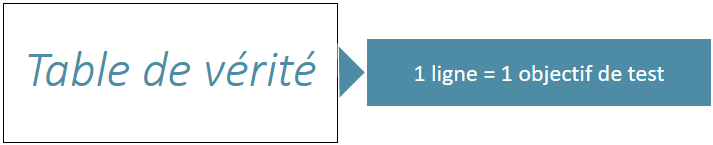
\includegraphics[width=0.8\textwidth]{./img/truth_table.png}
    \end{center}
\end{frame}

\begin{frame}
    \frametitle{Fonctionnalités}
    \begin{center}
        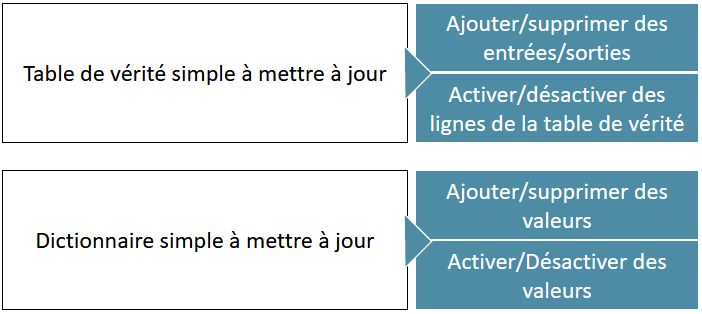
\includegraphics[width=0.8\textwidth]{./img/ttweb.png}
    \end{center}
\end{frame}